\documentclass[12pt]{article}

\usepackage{geometry}
\geometry{twoside, letterpaper, portrait}

\usepackage{emptypage}

\usepackage{amsmath}
\usepackage{siunitx}

\usepackage{graphicx}
\usepackage{float}
\usepackage{caption} 
\usepackage{wrapfig}

\usepackage{listings}

\usepackage{enumitem}

\usepackage{color}

\definecolor{comment_green}{rgb}{0,0.6,0}
\definecolor{light_gray}{rgb}{0.95,0.95,0.95}
\definecolor{med_gray}{rgb}{0.5,0.5,0.5}
\definecolor{string_mauve}{rgb}{0.58,0,0.82}

\usepackage{lipsum}

\usepackage{chngcntr}

\newcommand{\IIC}{I\textsuperscript{2}C }

\usepackage{csquotes}

\bibliographystyle{ieeetr} 

\lstset{ %
	backgroundcolor=\color{light_gray},   % choose the background color
	basicstyle=\scriptsize\ttfamily,    % the size of the fonts that are used for the code
	breakatwhitespace=false,         % sets if automatic breaks should only happen at whitespace
	breaklines=true,                 % sets automatic line breaking
	captionpos=b,                    % sets the caption-position to bottom
	commentstyle=\color{comment_green},    % comment style
	deletekeywords={...},            % if you want to delete keywords from the given language
	escapeinside={\%*}{*)},          % if you want to add LaTeX within your code
	extendedchars=true,              % lets you use non-ASCII characters
	frame=single,                    % adds a frame around the code
	keepspaces=true,                 % keeps spaces in text, useful for keeping indentation of code 
	keywordstyle=\color{blue},       % keyword style
	language=Octave,                 % the language of the code
	otherkeywords={*,...},           % if you want to add more keywords to the set
	numbers=none,                    % where to put the line-numbers; possible values are (none, left, right)
	numbersep=5pt,                   % how far the line-numbers are from the code
	numberstyle=\tiny\color{med_gray}\ttfamily, % the style that is used for the line-numbers
	rulecolor=\color{black},         % if not set, the frame-color may be changed on line-breaks within not-black text (e.g. comments (green here))
	showspaces=false,                % show spaces everywhere adding particular underscores; it overrides 'showstringspaces'
	showstringspaces=false,          % underline spaces within strings only
	showtabs=false,                  % show tabs within strings adding particular underscores
	stepnumber=1,                    % the step between two line-numbers. If it's 1, each line will be numbered
	stringstyle=\color{string_mauve},     % string literal style
	tabsize=4,	                     % sets default tabsize to 2 spaces
	title=\lstname                   % show the filename of files included with \lstinputlisting; also try caption instead of title
	morecomment=[l][\color{magenta}]{\#}
}


\begin{document}
	
% Set the counters to count by section
\counterwithin{figure}{section}
\counterwithin{lstlisting}{section}

\begin{titlepage}
	\centering
	
\includegraphics[width=0.20\textwidth]{figures/dal_logo.pdf}\par\vspace{1cm}
	{\scshape\LARGE Dalhousie University\par}
	\vspace{1cm}
	{\Large Report of Summer Work Term Project\par}
	{May 2 - August 26, 2016\par}
	\vspace{1cm}
	{\LARGE\bfseries Designing a Navigation Controller for an Autonomous Sailboat\par}
	\vfill
	{\itshape Performed at\par}
	{UW-STREAM Lab\par}
	{1340 Barrington Street\par}
	{Halifax, Nova Scotia\par}
	\vspace{0.5cm}
	{\itshape by\par}
	{\Large Thomas Gwynne-Timothy\par}
	\vspace{0.5cm}
	{\itshape in partial fulfillment of the requirements of the\par Engineering Co-operative Education Program}
	\vfill
	
	\vfill
	
	% Bottom of the page
	{\large September 13, 2016\par}
\end{titlepage}

\cleardoublepage

\pagenumbering{roman}
\setcounter{page}{1}

\section*{Summary}
\addcontentsline{toc}{section}{Summary}
\lipsum[1]

\cleardoublepage

\tableofcontents

\clearpage

\listoffigures
\addcontentsline{toc}{section}{List of Figures}

\clearpage

\section*{Acknowledgments}
\addcontentsline{toc}{section}{Acknowledgments}
The success of this project relied heavily on the talented team of engineers and technologists who helped design and build the sailboat. 

My supervisor, Dr. Jean-Francois Bousquet, provided valuable insight from last year's attempt at the Microtransat Challenge. He also help guide the boat's software architecture. 

Andrew Dobbin, a master's student in Dr. Bousquet's lab, helped design the sailboat's hardware and circuitry. He also assisted in testing and calibrating various hardware components onboard the boat. 

Julia Sarty, an undergraduate student, helped implement the sailboat's software. She developed a graphical user interface (GUI) to communicate with the sailboat via XBee radio. This system was critical during testing as it provided real-time data visualization and remote control over the sailboat's sail and winch.

Mark LeBlanc, the chief technologist for Dalhousie's Electrical \& Computer Engineering department, designed circuitry to connect sensors and devices to the sailboat's microcontroller. He also routed the printed circuit boards on which the sailboat's hardware was mounted.

Piotr Kawalec and Graham Muirhead, members of the team's mechanical group, built the physical sailboat. They manufactured the ship's hull, built motor drive systems for the rudder and sail, packaged and wired the boat's batteries, constructed waterproof connectors for the boat's electronics, and integrated all of these systems together into a seaworthy vessel. 

Dr. Rob Warner, a professor in Dalhousie's mechanical department, designed the boat's hull. He also provided a boat for the team to use during sea trials around Halifax.

Dr. Josh Leon, Dalhousie's Dean of Engineering, oversaw the project and ensured it had the resources it needed.

\clearpage

\pagenumbering{arabic}

\section{Introduction}
Nova Scotia has a long history of sailing, so its fitting that Dalhousie University -- the province's most prominent research institution -- is making an effort to lead the way in automating the ancient form of transport. Autonomous sailing has many potential applications, ranging from large, self-navigating yachts to small, data-collecting drones. A fleet of energy efficient ``sailbots'' could provide Dalhousie researchers with the data they need to study environmental phenomena and assess that state of our oceans. It is with these applications in mind that Dalhousie's Faculty of Engineering has set out to build an autonomous sailboat.

\begin{figure}[h]
	\centering
	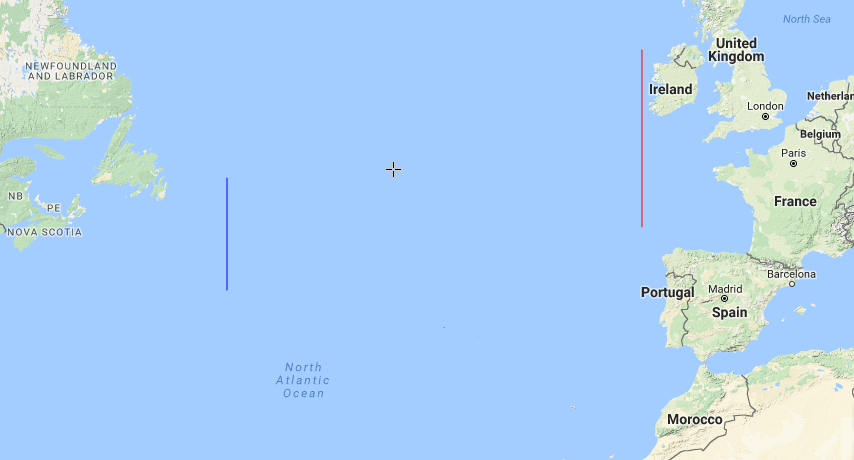
\includegraphics[width=0.7\textwidth]{figures/start_finish.png}
	\caption[Microtransat start and finish]{\textsl{Microtransat start (blue) and finish (red)} \cite{micro_map}}
	\label{fig:start_finish}
\end{figure}

The project is being driven by the Microtransat Challenge: ``a transatlantic race for autonomous boats.'' \cite{micro_main} The goal of the challenge is to promote the development autonomous sailboats and marine vehicles. Boats competing in the West to East group must pass a start line off the shore of NewfoundLand and cross the Atlantic Ocean to a finish line off of France (see Figure~\ref{fig:start_finish}). No team has every completed the challenge, which gives Dalhousie an opportunity to distinguish itself from other ocean research institutions. 

\subsection{Employer Background}
Dalhousie's Dean of Engineering, Dr. Josh Leon, assembled a team to focus on the autonomous sailboat project. The team was comprised of a group of mechanical engineers developing the physical boat and a group of electrical engineers developing the boat's control system. The electrical engineering group was pulled from Dalhousie's UW-STREAM laboratory, which designs hardware and software for underwater communication and sensing systems. My work on this project was completed as a member of this research group.

The UW-STREAM group is directed by Dr. Jean-Francois Bousquet. Dr. Bousquet joined Dalhousie's Electrical \& Computer Engineering Department in 2013. His research focuses on ``low-power integrated circuits applied to wireless communication,''\footnote{UW-STREAM site} but his research group also works on developing advanced signal processing algorithms for underwater acoustics and communication. Dr. Bousquet strives to implement his group's designs and perform real world tests and deployments.

\subsection{Problem Definition}
The problem assigned to me was to design and develop the software for the autonomous sailboat. This included developing drivers to interact with the sailboat's peripherals, control systems for the boat's electromechanical components, navigation algorithms to update the boat's course, and a basic operating system to manage these tasks.

\subsection{Scope of Report}
This report provides a summary of the design of the autonomous sailboat's software system. The architecture, as well as the operation of each separate software module, is described. The report focuses on the interfaces for each module and the relationships between the modules; however, the implementations of several key components are outlined. This report is not a complete documentation of the autonomous sailboat's software, but rather a summary of its design and structure.

The report does not include hardware design or component selection. These stages of the design were performed prior to my involvement in the project. The report does not document the design or manufacture of the physical boat. This was performed by a separate group in the team. 

The report's results section is limited because the sailboat's first tests were scheduled after the end of my work term. Testing of the sailboat should continue through September, so a more complete set of results will be available at the end of the month.

Should the reader be interested in learning more about the implementation of a particular component or see a full code listing, they are invited to contact me.

\clearpage

\section{Requirements}
The requirements for the autonomous sailboat were outlined at the outset of the project. They were developed using The Microtransat Challenge rules\footnote{http://microtransat.org/rules.php} and experience from the previous year's attempt at the competition. 

The project's most important requirement was to adhere to The Microtransat Challenge rules. Many of the rules apply to the physical design of the boat, and therefore were not immediately applicable to the software development team. The most relevant rules are related to navigation, communication, and tracking. The project was also constrained by existing design decisions. The microcontroller and sensor hardware had already been selected and purchased, so the software was required to work with these systems. 

\subsection{Navigation}
The sailboat must navigate autonomously. Before a competition attempt begins, the boat may be loaded with way points. Once the boat is released, it may no longer course or way point updates. It must create its own course based the preloaded way points, publicly broadcast data (such as weather forecasts), and/or onboard sensor readings.

\subsection{Control \& Communication}
The boat may only transmit data back to the team while its deployed. It may also receive publicly available signals and sense its environment with onboard sensors, but it may not receive data from the team. The boat cannot be remotely reprogrammed or reconfigured in any way. 

While these restrictions apply to the boat's final deployment, they don't need to be adhered to during testing. In fact, having remote control ability is an asset during sea trials, where manual adjustments to the sail and rudder could prevent faults in the navigation algorithm leading the boat astray and into danger. Last year's team noted that having a remote control for the boat proved essential to testing.

\subsection{Tracking \& Data Logging}
Data transmissions from the boat are not only allowed but required. The team must "provide their boat's position to the organisers via a web or email interface at least once every 6 hours."\footnote{ibid} Failure "to transmit for more than 10 consecutive days or a total of more than 15 days"\footnote{ibid} will result in disqualification. In addition to position, the boat can also transmit its status, including battery information, sensor readings, navigation status, and motor information.

While these data logs are useful for evaluating the boat's status during deployment, they have more value during testing where they can help identify bugs in the boat's software. Last year's team indicated that more data logs would have given much more insight into the boat's operation during tests, so this year's design was required to provide the following readings:
\begin{itemize}
	\setlength\itemsep{0.15em}
	\item GPS coordinates
	\item Wind speed and direction
	\item Compass heading, pitch, and roll
	\item Current way point coordinates and threshold radius
	\item Distance and bearing to current way point
	\item Course set by navigation algorithm
	\item Rudder and sail positions set by navigation algorithm
\end{itemize}

\subsection{Hardware Interfaces}
As the project was introduced, several important design decisions had already been made. The sailboat would use a SAMD20 microcontroller from Atmel, which features an ARM Cortex-MO processor. The sailboat would also use a MTK3339 GPS module, an LCJ Capteurs CV-7 wind sensor, and an HMC6343 compass. Electrical \& Computer Engineering's chief technologist, Mark LeBlanc, already designed and printed circuits to interface these devices with the microcontroller. Working with this pre-designed hardware configuration was an important requirement for the sailboat's software.

\clearpage

\section{Design}
The sailboat's software has a hierarchical structure with three layers: control, task, and input/output (i/o). The control layer manages the state of the sailboat and runs various tasks at periodic intervals. The task layer contains high-level modules that manage the sailboat's peripherals. It provides a streamlined interface to the underlying input/output layer, which handles low-level code to the microcontroller's hardware interfaces. A visual overview of the layered architecture is shown below in Figure~\ref{fig:module_hierarchy}.  

\begin{figure}[h]
	\centering
	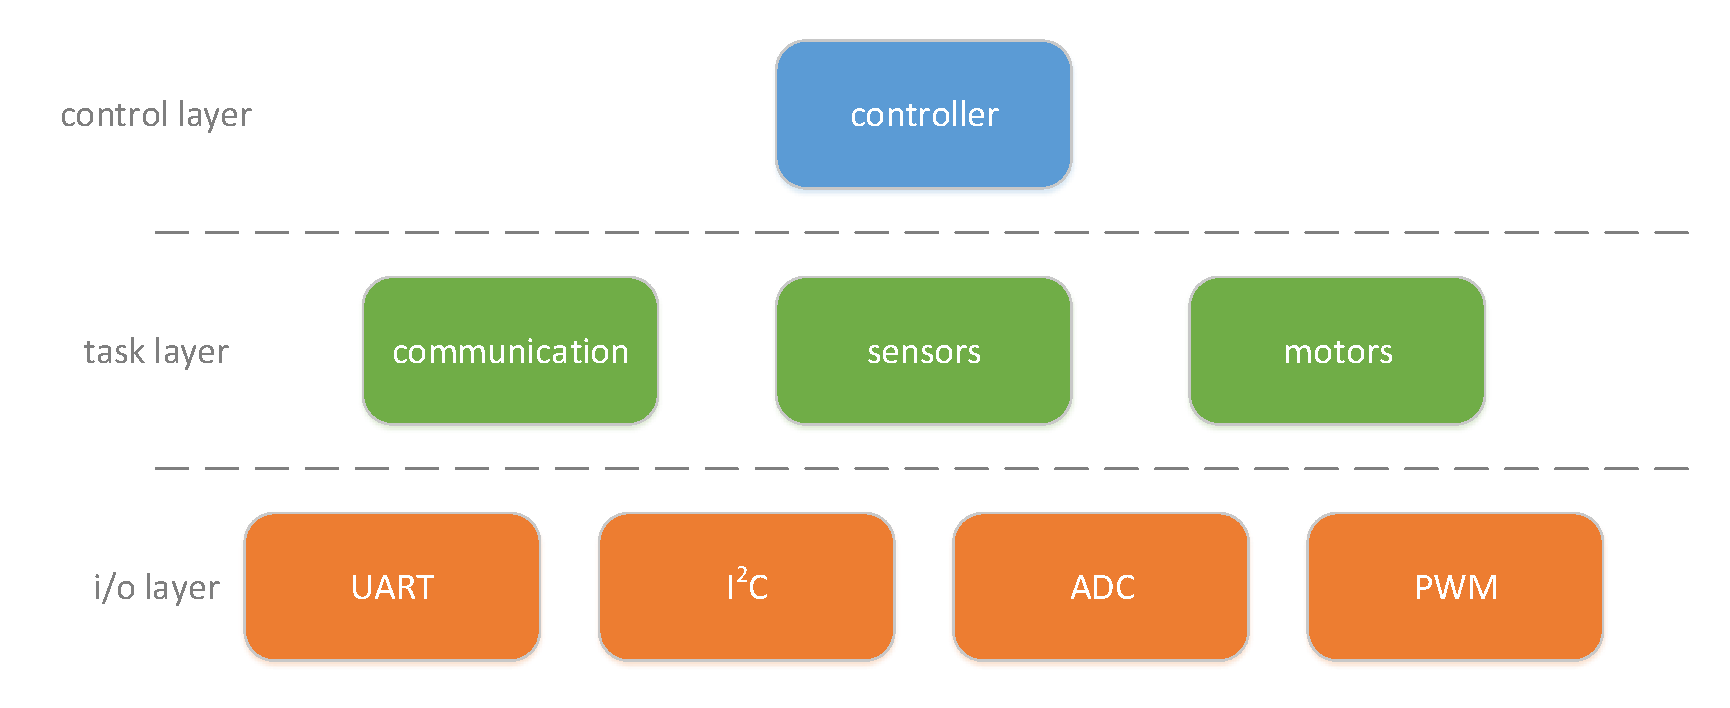
\includegraphics[width=\textwidth]{figures/module_hierarchy.pdf}
	\caption[Module hierarchy]{\textsl{Module hierarchy}}
	\label{fig:module_hierarchy}
\end{figure}

The modular structure has several benefits. Most importantly, it separates the hardware specific drivers from the high-level logic. Moving the project to another hardware platform would only require changes to the i/o layer, while the control and tasks layers could stay the same. The primary drawback of this architecture is that it requires significant design and planning. The responsibilities of each module and layer must be distinguished before implementation can begin.

\subsection{Control Layer}
\label{subsec:ctrl}
The control layer manages the state of the sailboat and its peripherals. It is responsible for running tasks critical to the sailboat's operation and sharing data between these tasks.

The controller uses a clock to manage the sailboat's periodic tasks. Each task is given a timestamp, and when the clock exceeds the time stamp, the task is initiated. Upon completion of the task, the time stamp is incremented by the task's period. This structure is highly flexible, allowing fine control over the timing between tasks. 

The tasks are designed such that they finish within the timer period (\SI{200}{\milli\second}); however, this is not guaranteed. Many of the tasks interact with the sailboat's peripherals, which could fail. The drivers for communicating with these devices (described in Section~\ref{subsec:io}) have safeguards to protect against device failures, but faults are still possible. In the case that a task becomes unresponsive and fails to return, a watchdog timer will force a software reset. The watchdog timer is started at the same time as the main control timer. With each tick of the control timer, the watchdog is "kicked". Otherwise, the watchdog timer will overflow, and a software reset will occur. Upon the reset, the status of each peripheral is checked and the control loop restarts.

The process for running tasks described above is handled by the timer tick callback. This function is called each time the control timer overflows. The function's implementation is shown in Listing~\ref{list:timer_tick}.

In addition to managing tasks, the control layer is also responsible for maintaining the state of the sailboat. The sailboat's state is partially derived from the state of its peripherals. The peripherals are each assigned one of three states: enabled, disabled, or inoperative. Meanwhile, the sailboat controller itself has states, which can be changed by the user at runtime via radio. 

The first state is the \textit{operational mode}, which dictates which tasks the sailboat will perform. There are three operational modes: autonomous, remote, and way point load. In autonomous mode, the controller calls upon its navigation routines to select appropriate rudder and sail positions to send the boat towards the target way point (see Section~\ref{subsubsec:nav}). In remote mode, the controller adjusts the motors in response to control messages sent via radio. In way point load mode, the controller listens for arriving way point messages and loads them into the EEPROM.

The second state is the \textit{data log mode}, which dictates how data log messages will be transmitted. There are two modes: deploy and test. In deploy mode, data log messages are sent every hour through the Xeos satellite transmitter channel. In test mode, data log messages are sent frequently over the Xbee radio channel. The data log period for testing is configurable, but it typically ranges between \SI{1}{\second} and \SI{60}{\second}. The message protocol and format are described in Section~\ref{subsubsec:comm}.

\subsection{Task Layer}
The system's task layer is responsible for providing a high-level interface for each of the sailboat's core functions. The task layer allows the control layer to communicate with the sailboat's peripherals without having to interact directly with low level drivers, which are described in Section~\ref{subsec:io}. The tasks are listed below.

\begin{itemize}
	\setlength\itemsep{0.15em}
	\item Data logging
	\item GPS reading
	\item Wind vane reading
	\item Compass reading
	\item Rudder control
	\item Course selection
\end{itemize}

\subsubsection{Data Logging \& Communication}
\label{subsubsec:comm}
One of the most important requirements for this project was to implement an effective data logging system for the sailboat. This is critical for effective testing and successful deployment. The sailboat must log sensor data, including GPS coordinates, wind information, and compass readings. It must also log controller data, such as the bearing to the next way point, the course selected by the navigation algorithm, and the rudder and sail positions. 

The sailboat has two data logging modes - \textit{test} and \textit{deploy}. In test mode, the data is sent frequently over short range radio. The system uses an Xbee Series 1 radio module that provides a point-to-point serial interface with a matching XBee module connected to a host computer. The data can be visualized in real-time with a graphical user interface (GUI) program created by another student working on this project. The GUI can also log the data to a file for analysis later. In deploy mode, the data is sent infrequently via a satellite transmitter. The sailboat is equipped with a Xeos Onyx device that can communicate over the Iridium network. The Xeos device provides a serial interface through which data can be logged to a remote server. These log messages can be viewed through a web client provided by Xeos. 

The GUI application for viewing and logging data can also be used to control and configure the sailboat. To facilitate this, a custom message format was created. The format uses the same style as the National Marine Electronics Association (NMEA) format used by the GPS and wind vane modules. The format uses a header that indicates message structure, followed by an ID that indicates the type of data the message carries. After the ID, a list of data fields are sent. The message is then terminated with a checksum. A generic message is shown below.

\begin{center}
	\texttt{\$DALSAIL,<id>,<arg1>,...,<argn>*checksum}
\end{center}

There are currently 11 different message IDs. As the project evolves, more may be added. The existing message types are described below.

\paragraph{Message acknowledgment (\texttt{000}):}
These messages have only one field - the message acknowledgment type. The acknowledgment type can indicate one of four things: a received message was handled successfully (0), a received message was not handled successfully (1), a received message was found to be corrupt (2), or a received message resulted in no change (3). An example acknowledgment indicating a success is shown below.
\begin{center}
	\texttt{\$DALSAIL,000,0*5e}
\end{center}

\paragraph{Mode change (\texttt{001}):}
These messages change the sailboat's operational mode (described in Section~\ref{subsec:ctrl}). The message has one field, which indicates a mode change to either autonomous mode (0), remote mode (1), or way point load mode (2). An example message requesting a change to remote mode is shown below.
\begin{center}
	\texttt{\$DALSAIL,001,1*5e}
\end{center}

\paragraph{Data log mode change (\texttt{002}):}
These messages change the sailboat's data log mode (described in Section~\ref{subsec:ctrl}). The message has one field, which indicates a mode change to either deploy mode (0) or test mode (1). An example message requesting a change to deploy mode is shown below.
\begin{center}
	\texttt{\$DALSAIL,002,0*5c}
\end{center}

\paragraph{Remote motor control (\texttt{003}):}
These messages can be sent when the sailboat is in remote mode. They have two fields that set the rudder and sail positions. The rudder controls the direction of the boat and can be set between \SI{-45}{\degree} and \SI{45}{\degree}. The sail can be pulled in tight or let out loose to take advantage of the wind by setting the boom angle between \SI{10}{\degree} and \SI{65}{\degree}. An example message that sets the rudder to \SI{12}{\degree} and the sail to \SI{30}{\degree} is shown below.
\begin{center}
	\texttt{\$DALSAIL,003,12,30*41}
\end{center}

\paragraph{Way point entry (\texttt{004}):}
These messages can be sent when the sailboat is in way point load mode. They have fields that indicate the way point index, the GPS coordinates of the way point, the way point's threshold radius, and the index of the next way point in the path. Message parsing is made easier by scaling small decimal numbers to remove the decimal point but maintain precision. The GPS coordinates (in decimal degrees) require 6 decimal places of precision, so they are scaled up by a factor of \SI{1000000}{} -- effectively converting the units to micro degrees. An example message containing a path's third (index origin = 0) and final way point is shown below. The coordinates are (\SI{44.123456}{\degree}, \SI{-65.123456}{\degree}) with a threshold radius of \SI{500}{\meter}. The next way point index is set to 0 to indicate that the sailboat should loop back to the first way point when it completes the path.
\begin{center}
	\texttt{\$DALSAIL,004,2,44123456,-65123456,500,0*73}
\end{center}

\paragraph{Data log rate change (\texttt{005}):}
These messages change the rate at which data is logged in test mode (data logs sent via XBee radio). This message has a single field indicating the time between messages, in seconds. The value must be between \SI{1}{\second} and \SI{60}{\second}. The example message below sets the data log period to \SI{5}{\second}.
\begin{center}
	\texttt{\$DALSAIL,005,5*5e}
\end{center}

\paragraph{GPS data log (\texttt{006}):}
These messages are sent from the sailboat to log the most recent GPS reading. The messages contain the decimal degree coordinates of the last reading. They are integers, in units of micro degrees. The example message below shows a log of a reading (\SI{45.231467}{\degree}, \SI{-67.231467}{\degree}).
\begin{center}
	\texttt{\$DALSAIL,006,45231467,-67231467*69}
\end{center}

\paragraph{Wind vane data log (\texttt{007}):}
These messages are sent from the sailboat to log the most recent wind vane reading. The message contains the wind speed and angle. The angle is represented in tenths of a degree relative to North, and the speed is represented in tenths of a meter per second. The example message below shows a reading with an angle of \SI{165.2}{\degree} at a speed of \SI{3.6}{\meter\per\second}. 
\begin{center}
	\texttt{\$DALSAIL,007,1652,-36*6d}
\end{center}

\paragraph{Compass data log (\texttt{008}):}
These messages 
\paragraph{Navigation status log (\texttt{009}):}
\paragraph{System reset cause (\texttt{010}):}


\subsubsection{GPS}
The sailboat uses a MTK3339 GPS module to track its position. The module uses a serial interface to transmit coordinates and receive control messages. At the task layer, an interface was designed to enable the module and get the most recent reading from it. The interface is shown in Listing~\ref{list:gps_interface}.

The GPS software module relies on the UART module (described in Section~\ref{subsubsec:uart}) and an NMEA module (used for parsing the data fields and validating the message checksum). The UART module is responsible to receiving messages and loading them into a buffer. The NMEA module is responsible for extracting messages from the buffer and stripping away the header and checksum. When \texttt{GPS\_GetReading()} is called, the GPS software module extracts messages from the buffer until there are no more complete messages available. It parses the most recent message and sends the data back in the provided data structure referenced by the \texttt{reading} argument. The status of this process is returned by the function.

\begin{wrapfigure}{R}{0.55\textwidth}
	\centering
	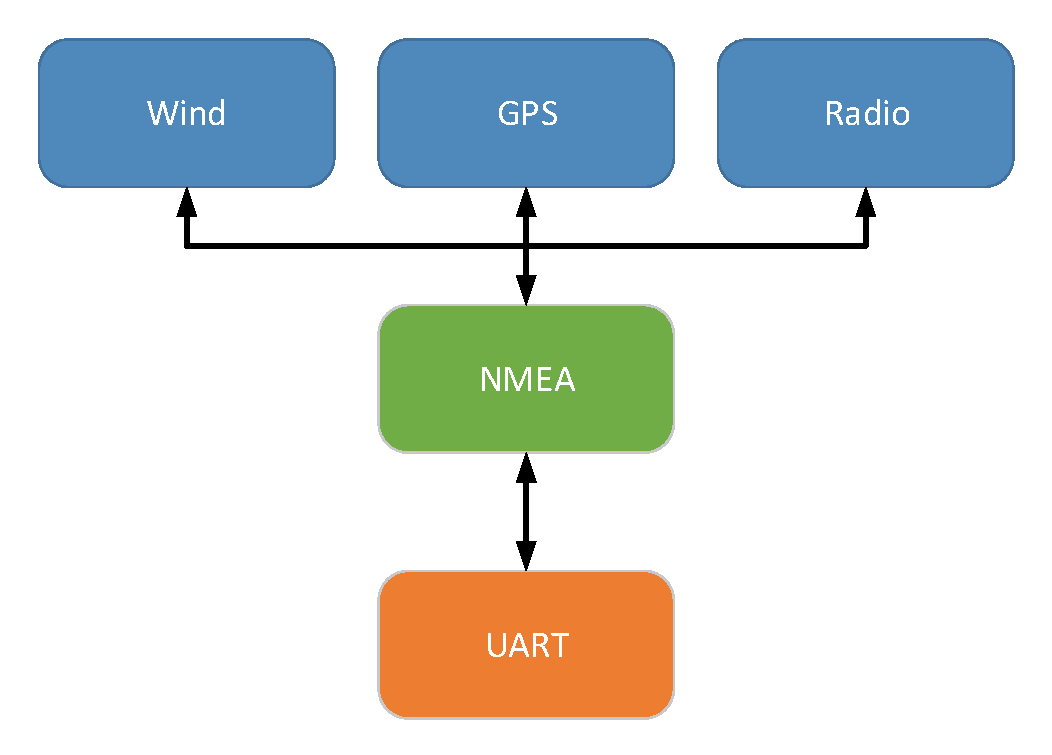
\includegraphics[width=0.55\textwidth]{figures/comm_stack.pdf}
	\caption[Serial communication hierarchy]{\textsl{Serial communication hierarchy}}
	\label{fig:comm_stack}
\end{wrapfigure}

The relationship between the GPS software controller and its underlying software modules is shown in Figure~\ref{fig:comm_stack}. This hierarchy is shared between the tasks that depend on serial communications with NMEA compliant devices, namely the wind vane and the XBee radio.

\subsubsection{Wind Vane}
The sailboat's LCJ Capteurs CV-7 ultrasonic wind sensor operates much like the GPS, and its software interface is nearly identical. As readings arrive, the UART driver queues them in a buffer. When the control layer requests the most recent reading, the wind module uses the NMEA module to extract the messages and remove the overhead. The most recent message is parsed and returned to the caller. The wind vane interface is shownb in Listing~\ref{list:wind_interface}.

\subsubsection{Compass}
The sailboat is also equipped with an HMC6343 compass. The compass provides the boat's heading, pitch, and roll. It can also measure acceleration. The compass differs from the other sensors in that uses an \IIC interface. Whereas the wind vane and GPS sensors provide a steady stream of data, the compass only sends data when it receives a read command. The compass shares the the \IIC bus the with an EEPROM module.

The compass interface provides functions for enabling and disabling the device, as well as making a variety of readings. The compass also features a built-in calibration sequence, so the interface provides functions to start and stop this routine. The full software interface is shown below in Listing~\ref{list:comp_interface}.

\subsubsection{Motors}
The sailboat has two motors that drive the rudder shaft and sail winch. The motors selected by the hardware team feature on-board speed controllers and encoder feedback. The hardware team augmented the motors with worm-drive assemblies that mitigate backdrive and rotary potentiometers that provide direct angle feedback. The software team was tasked with developing a controller for setting the rudder angle and sail tension.

\begin{figure}[h]
	\centering
	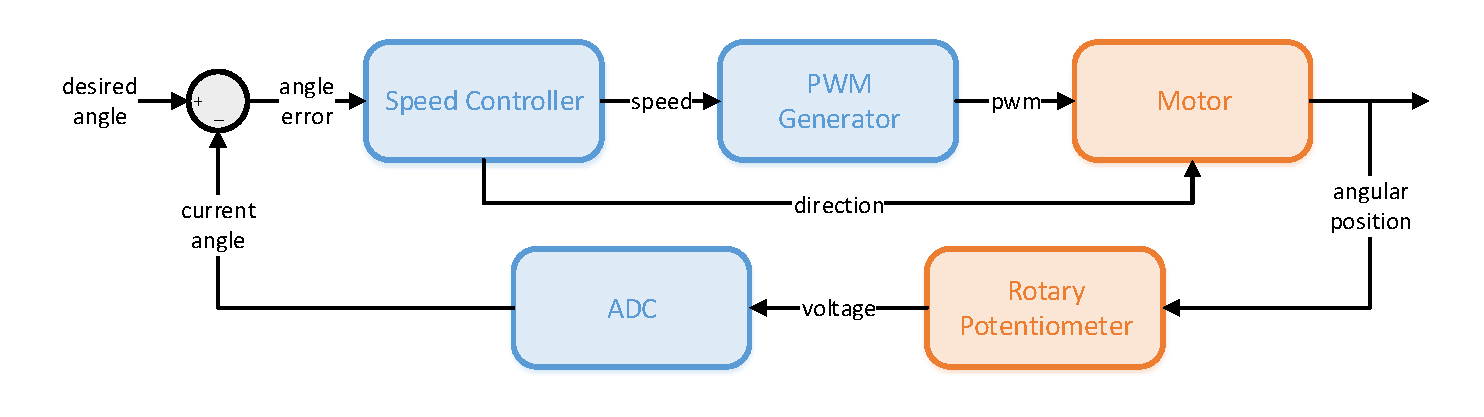
\includegraphics[width=\textwidth]{figures/motor_block.pdf}
	\caption[Block diagram of motor controller]{\textsl{Block diagram of motor controller}}
	\label{fig:motor_block}
\end{figure}

The role of the software controller is highlighted in the block diagram shown in Figure~\ref{fig:motor_block}. The controller relies on two hardware drivers: the PWM generator and the ADC module. The PWM generator is responsible for converting a motor speed value to a PWM signal that can be sent to the motor's speed controller. The ADC module is responsible for measuring the voltage at the rotary potentiometer, which can be mapped to an angular position. These drivers are discussed in Section \ref{subsec:io}.

The speed controller block uses proportional control to map the angle error to a motor speed (PWM duty cycle). The transfer function is clamped such that a minimum speed is used when the angle error drops below \SI{5}{\degree} and a maximum speed is used when the angle error exceeds \SI{20}{\degree}. The transfer function has been plotted in Figure~\ref{fig:controller_transfer}.

\begin{wrapfigure}{R}{0.55\textwidth}
	\centering
	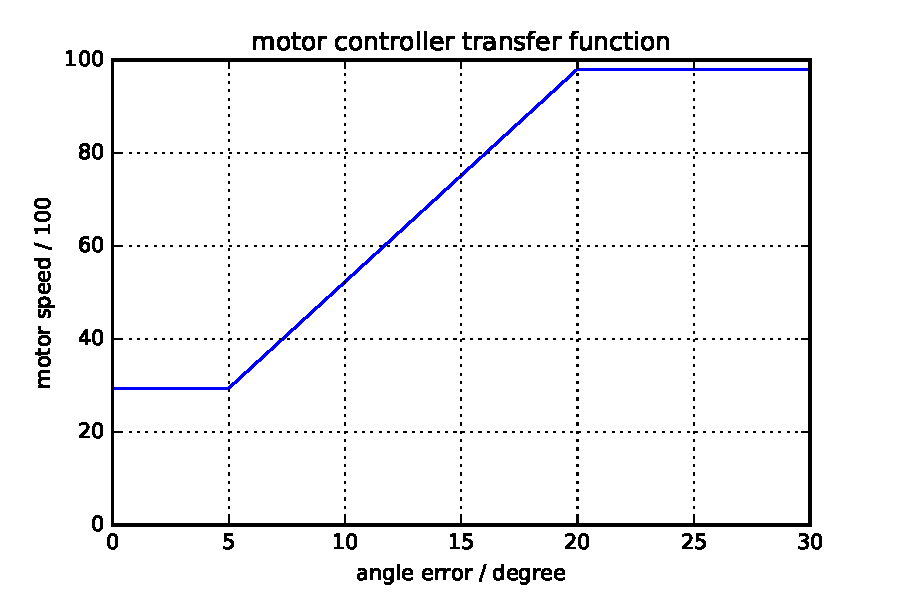
\includegraphics[width=0.55\textwidth]{figures/p_control.pdf}
	\caption[Speed controller transfer function]{\textsl{Speed controller transfer function}}
	\label{fig:controller_transfer}
\end{wrapfigure}

The motor control system was tuned empirically. This was sufficient because the motors are geared for a slow operational speed. Furthermore, the controller has logic to turn off the motors when the angle error falls below a  threshold of \SI{2}{\degree}. The slow speed of the motors and the low accuracy requirements on the rudder and winch angles permit such a simple control scheme. Systems that operate at higher speeds with greater accuracy requirements would demand a more rigorous design approach.

\subsubsection{Navigation}
\label{subsubsec:nav}
The last - and perhaps most critical - task is navigation. The navigation algorithm uses data from each of the sensors, as well as way points stored in the boat's EEPROM, to update the rudder and sail. The way points are loaded into the EEPROM via radio at the beginning of a mission and define the path the boat should follow. Each way point has a threshold radius, and when the distance between the boat's position and the way point falls within the threshold, a counter is incremented. After five consecutive GPS readings within the radius, the boat marks the way point complete and sets its course for the next one. The way points are stored in EEPROM to ensure the controller maintains its progress in the event of power loss.

\begin{wrapfigure}{L}{0.5\textwidth}
	\centering
	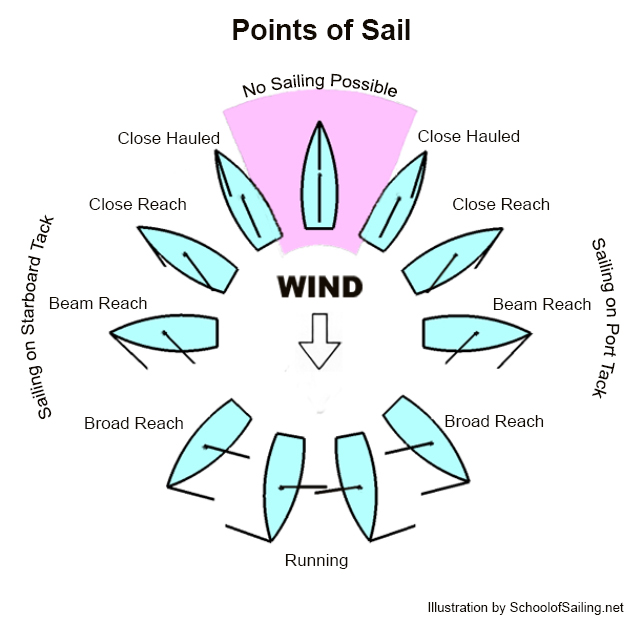
\includegraphics[width=0.5\textwidth]{figures/points_of_sail.jpg}
	\caption[Points of sail]{\textsl{Points of sail}}
	\label{fig:sail_pos}
\end{wrapfigure}

The navigation system must perform two main tasks: selecting a course to get to the target way point and updating the rudder to maintain that course. In general, the course can be selected as the bearing between the boat's current position and the target way point. However, the wind conditions may yield this course inefficient or infeasible. In situations where the wind direction is directly against this course, the boat must tack back and forth to make forward progress. In cases where the wind is directly behind the boat's course, it must jibe to maintain broad reach, which can be much faster than running directly with the wind.\footnote{http://www.schoolofsailing.net/points-of-sail.html} A visualization of the different sail positions with respect to the wind is shown in Figure~\ref{fig:sail_pos}.

The sailing algorithm accounts for tacking and jibing by first computing the course directly towards the way point and then applying offsets to this course based on the wind direction. If the course falls into the \textit{dead zone} (marked in pink in Figure~\ref{fig:sail_pos} and defined by \SI{45}{\degree} to either side of the wind direction), the the course will be updated to allow \textit{close hauled} sailing on the edge of the dead zone closest to the direct course. Similarly, if the direct course requires \textit{running}, the an offset will be applied to let the boat sail at \textit{broad reach}. Once the final course has been set, the navigation algorithm can output a sail position based on the direction of the wind. The boat uses five discrete sail positions corresponding to close hauled, close reach, beam reach, broad reach, and running. The sail position is then applied with the motor control task.

Once a course and sail position have been set, the boat must maintain that course. This is the responsibility of the rudder. The rudder control algorithm runs frequently at \SI{200}{\milli\second} intervals, comparing the heading from the compass to the target course. The difference is mapped to a rudder setting, which is then applied by the motor controller.

\subsection{Input/Output Layer}
\label{subsec:io}
The input/output layer contains device drivers for various hardware interfaces on board the SAMD20 microcontroller. These include the universal asynchronous receiver/transmitter (UART), the I\textsuperscript{2}C bus, the analog-to-digital converter (ADC), and the pulse-width modulation (PWM) generator. Each device driver makes use of the Atmel Software Framework, which provides utility functions and data structures for manipulating the SAMD20's registers. The following subsections describe the interface of each device driver.

\subsubsection{UART}
\label{subsubsec:uart}
The UART driver provides functions to facilitate communication over the SAMD20's four active transceivers. The four instances are mapped to the specific peripherals: an MTK3339 GPS receiver, a CV7 ultrasonic wind sensor, an XBee S1 Pro radio module, and a Xeos Onyx satellite transceiver.

The UART driver uses non-blocking, interrupt based functions. When the caller uses the transmit functions, which can send individual bytes or entire strings, the data is placed into buffer that gets emptied by the transmitter's interrupt service routine (ISR). The receive functions behave similarly. The caller must first enable the receiver. Once enabled, an ISR will push bytes into a circular first-in-first-out (FIFO) buffer as they arrive. When data is available, the UART driver's receiving functions will return a specific status code. This allows the caller to poll the receiver and pull data from the FIFO buffer when it becomes available. The non-blocking nature of the UART interface makes it well suited for the main controller's task system, which demands that tasks finish within \SI{200}{\milli\second}.

\subsubsection{\IIC}
The \IIC driver provides read and write functions for the boat's two \IIC slaves: the HMC6343 compass and the AT24C512 external EEPROM module. Because the \IIC devices must be commanded to transmit data, the \IIC driver uses a blocking interface for its commands. This is means that when the caller sends a read or write request, the function will not return until the request has been processed. This interface poses a risk to the task manager, as a function call could take longer than the \SI{200}{\milli\second} time slice given to each task. The compass and EEPROM operate at a \SI{100}{\kilo b \per\second} bus speed and a maximum typical latency of \SI{10}{\milli\second}, so hundreds of bytes can be written during a single task interval without approaching the time slice limit. However, a device fault could prevent this. Fortunately, the ASF library provides utility functions to determine when a device becomes unresponsive. An error code will be returned and passed up through the call stack to the task layer code that called the \IIC driver. Should an error go uncaught, the watchdog timer serves as a last resort to ensure the system does not become unresponsive. 

\subsubsection{ADC}
The SAMD20 features 16 analog pins, but the sailboat only needs two to measure the voltage at the sail and rudder potentiometers. Again, the ASF provides utilities to configure the ADC module and initiate conversions. The driver module wraps these routines into a simple interface for the task layer to use. The module provides one function to configure and initialize the ADC peripheral and another to perform an analog read. The read function is blocking, but the ADC is capable of sampling at \SI{350}{\kilo\hertz} -- orders of magnitude higher than the \SI{100}{\hertz} sampling rate of the motor control system.

\subsubsection{PWM}
The last module in the i/o layer is the pulse-width modulation driver. This module serves to generate signals to control the speed of the boat's rudder and sail motors. The driver makes use of the ASF timer-counter library to configure the PWM timers and control the frequency and duty cycle of the output signals. The interface exposed to the control layer provides functions to enable or disable the PWM channels and set their duty cycles independently. 
\clearpage

\section{Testing \& Results}

\begin{wrapfigure}{R}{0.5\textwidth}
	\centering
	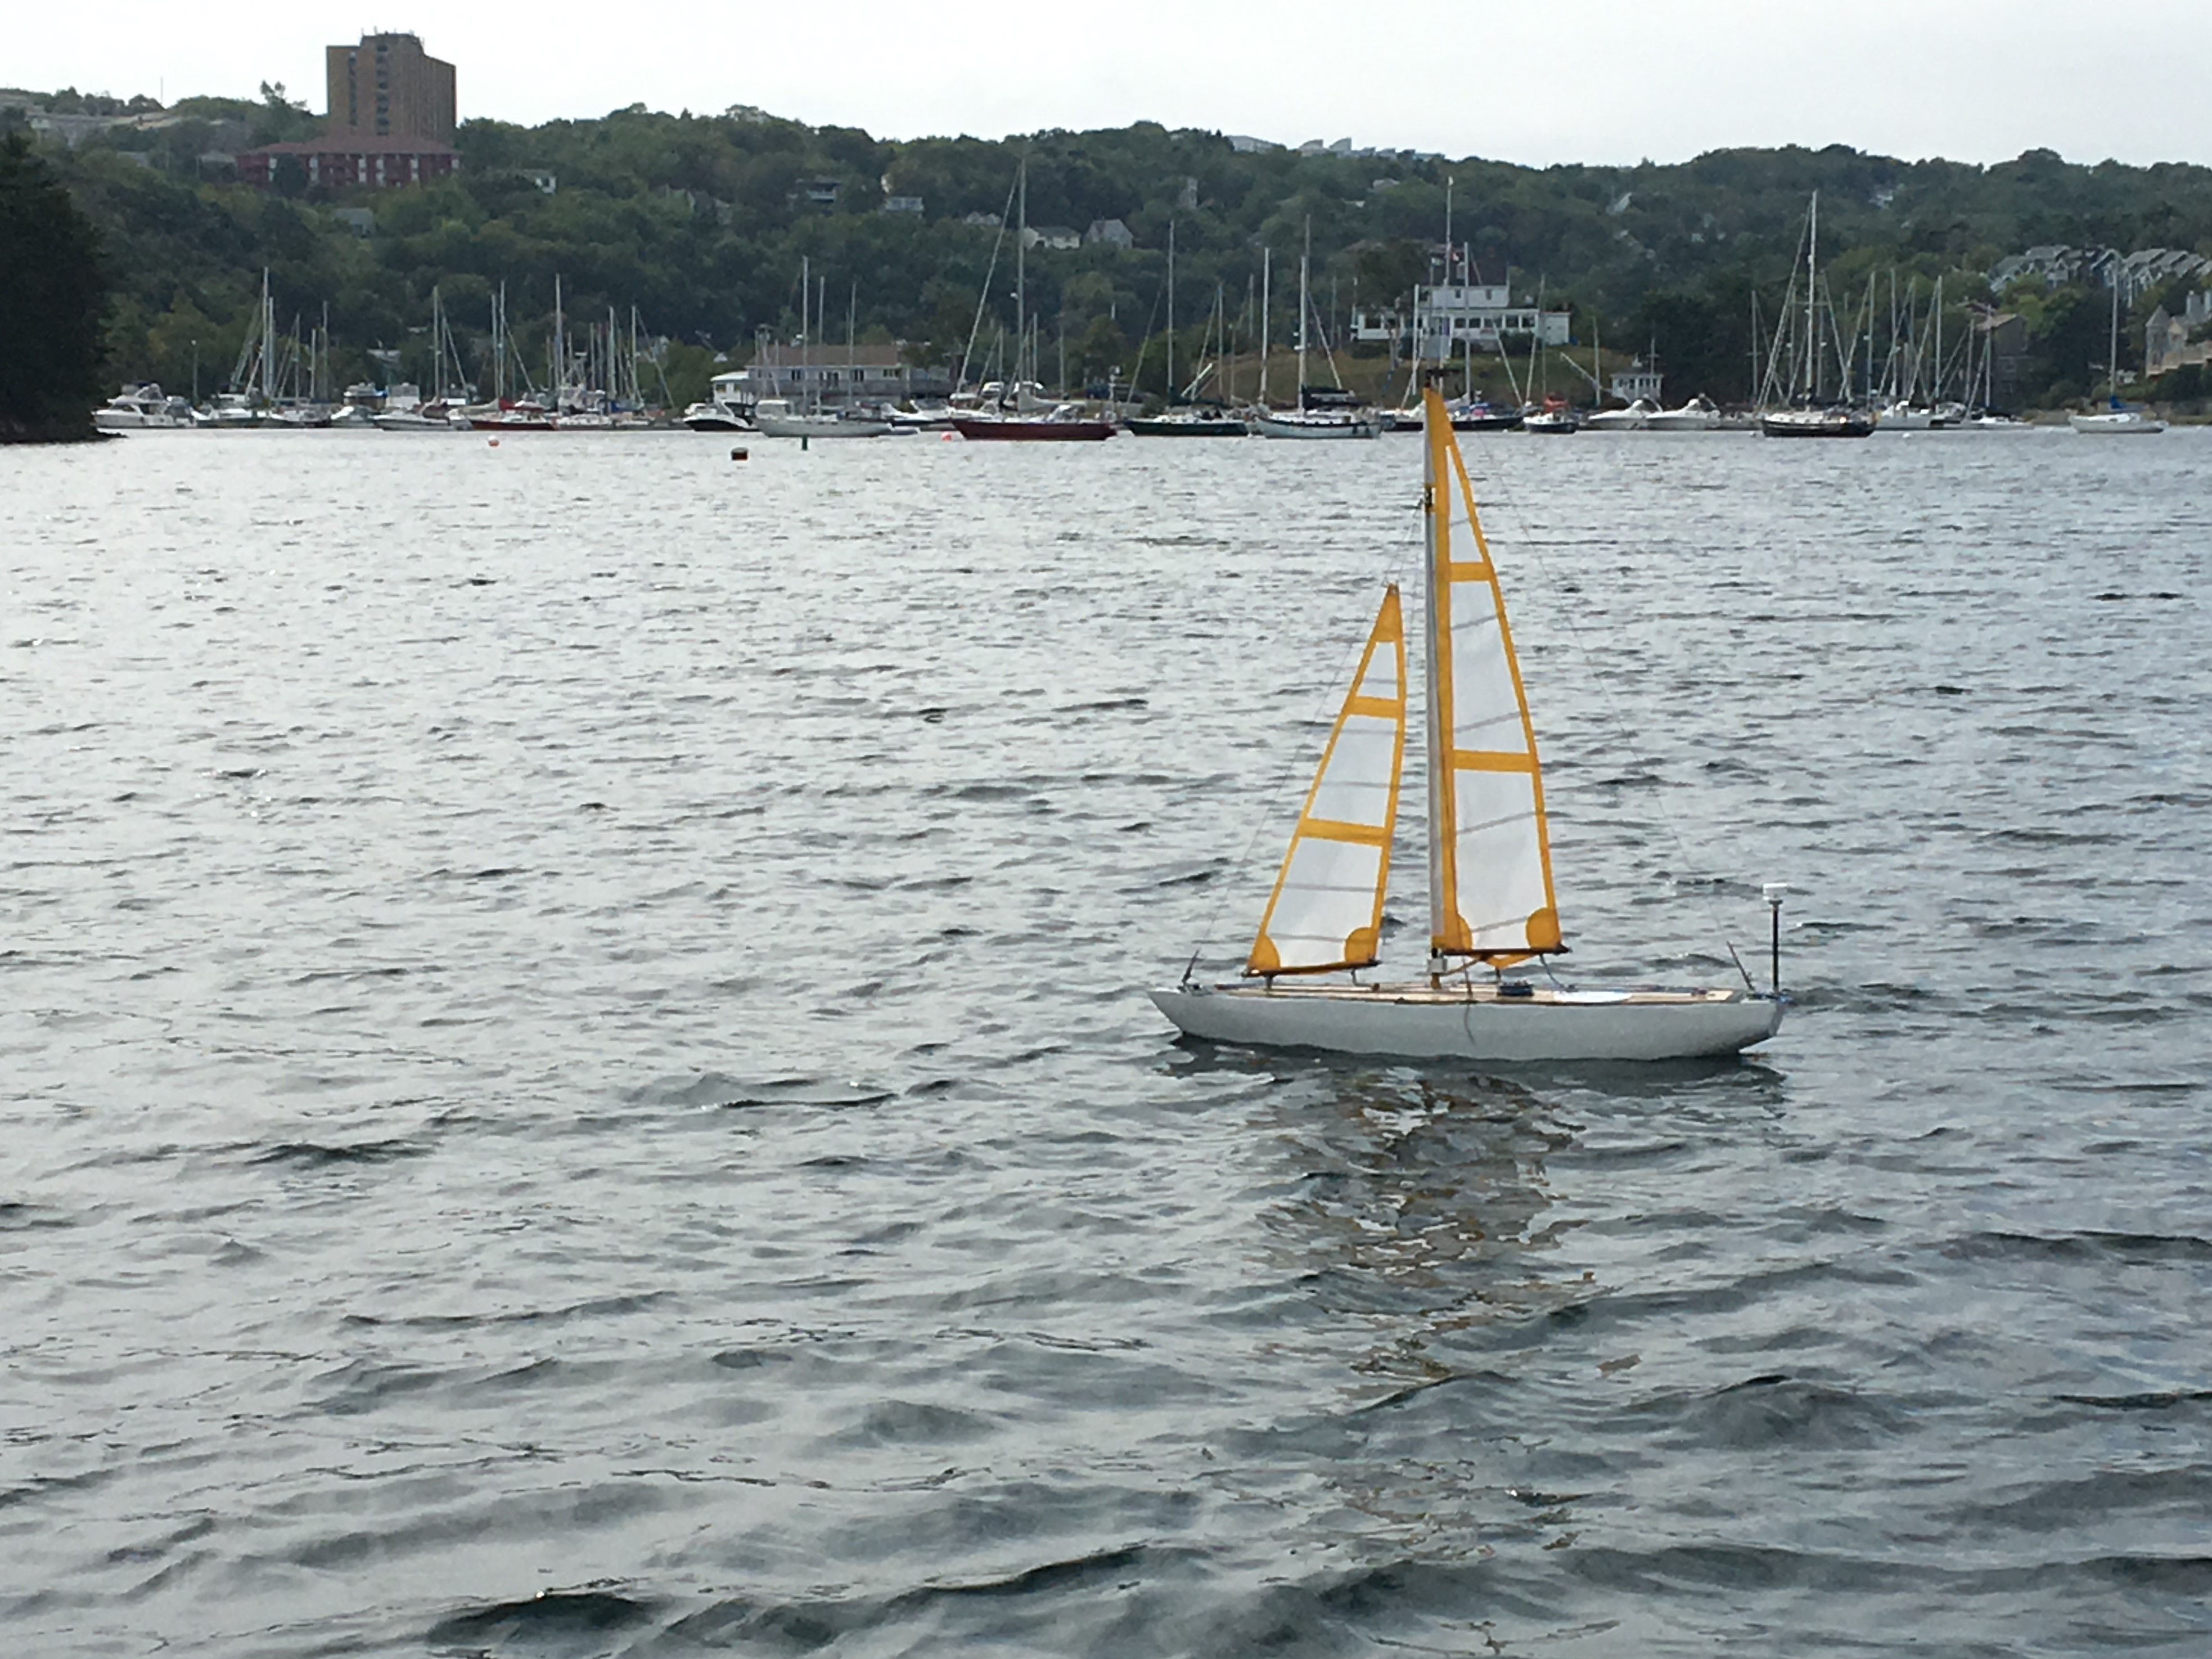
\includegraphics[width=0.5\textwidth]{figures/sailboat_test.jpg}
	\caption[Sailboat testing in the Arm]{\textsl{Sailboat testing in the Arm}}
	\label{fig:sail_test}
\end{wrapfigure}

The sailboat is currently beginning the integration testing stage of its development. It underwent its first sea trial on September 9, 2016, in Halifax's Northwest Arm, and while data from this deployment is still being processed, the test was a major success. This section of the report will focus on the testing procedures employed throughout the sailboat's development during the summer.

The development of the sailboat's software was test-driven. Headers for each module were created to define the interface for each component. Once the interface was designed, a test harness was created to validate the operation of each module. Once the header and tests were defined, the module's implementation could be completed. This development style worked well at the outset of the project, but it became challenging to follow as the project grew. It would have been easier to maintain with more developers working on the project. 

The sailboat's software was built from the i/o layer up. The first module to be completed was the UART driver, as this allowed debug messages to be transmitted from the sailboat controller to a host computer. From here, drivers for peripherals and sensors were implemented. The control layer was the final module to be completed as it required integrating each of the lower level components. Each sub-component was thoroughly tested before integration could begin.

To test the integrated software, a fake ``mission'' was created around Dalhousie's Sexton campus. Way points were created throughout the campus's parking lots and driveways (see Figure~\ref{fig:sexton_path}). The sailboat's internal hardware was loaded onto a cart (see Figure~\ref{fig:sail_cart}), which was pushed along the mission path. Meanwhile, data logs were transmitted to a host computer via XBee radio. The test's purpose was to verify that the sailboat could navigate through its list of way points. Compass and GPS readings were validated against reference data from other devices. These tests were helpful in revealing errors in navigation logic, but they were not useful in validating the rudder and sail control code. These aspects of the control system will be tested through sea trials in September 2016.

\begin{figure}[h]
	\centering
	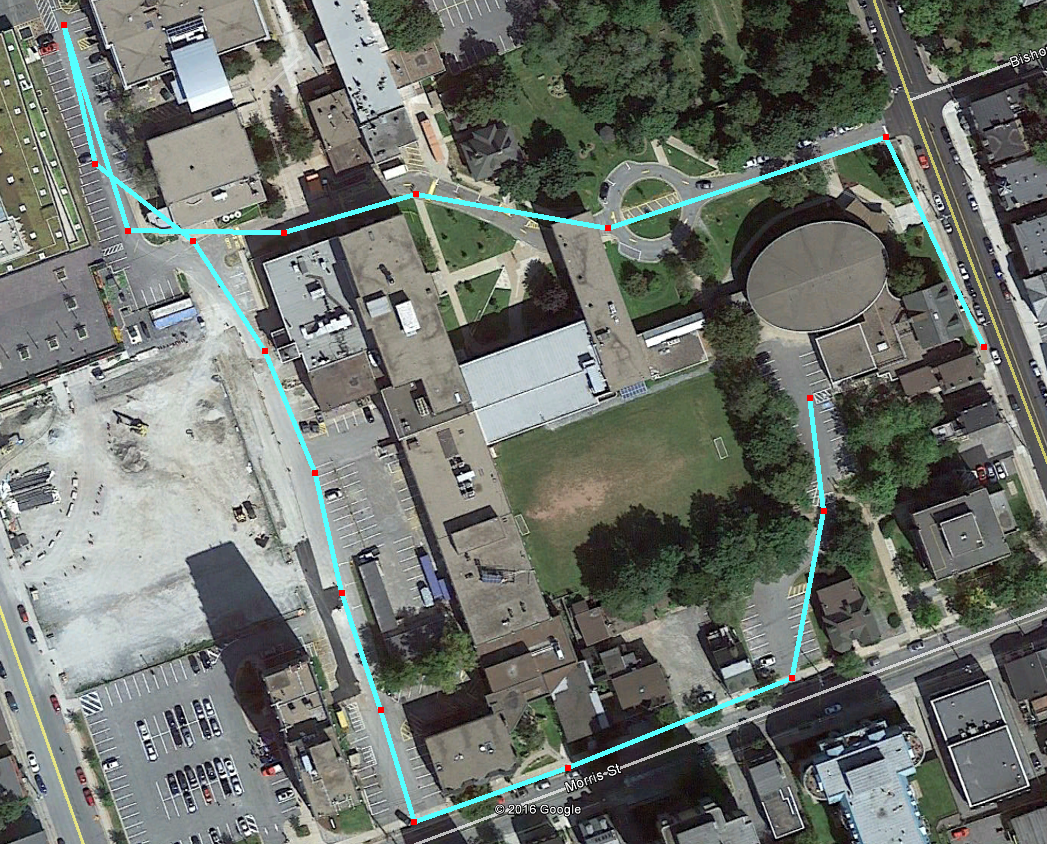
\includegraphics[width=0.7\textwidth]{figures/sexton_path.png}
	\caption[Sexton campus test path]{\textsl{Sexton campus test path}}
	\label{fig:sexton_path}
\end{figure}

\begin{figure}{h}
	\centering
	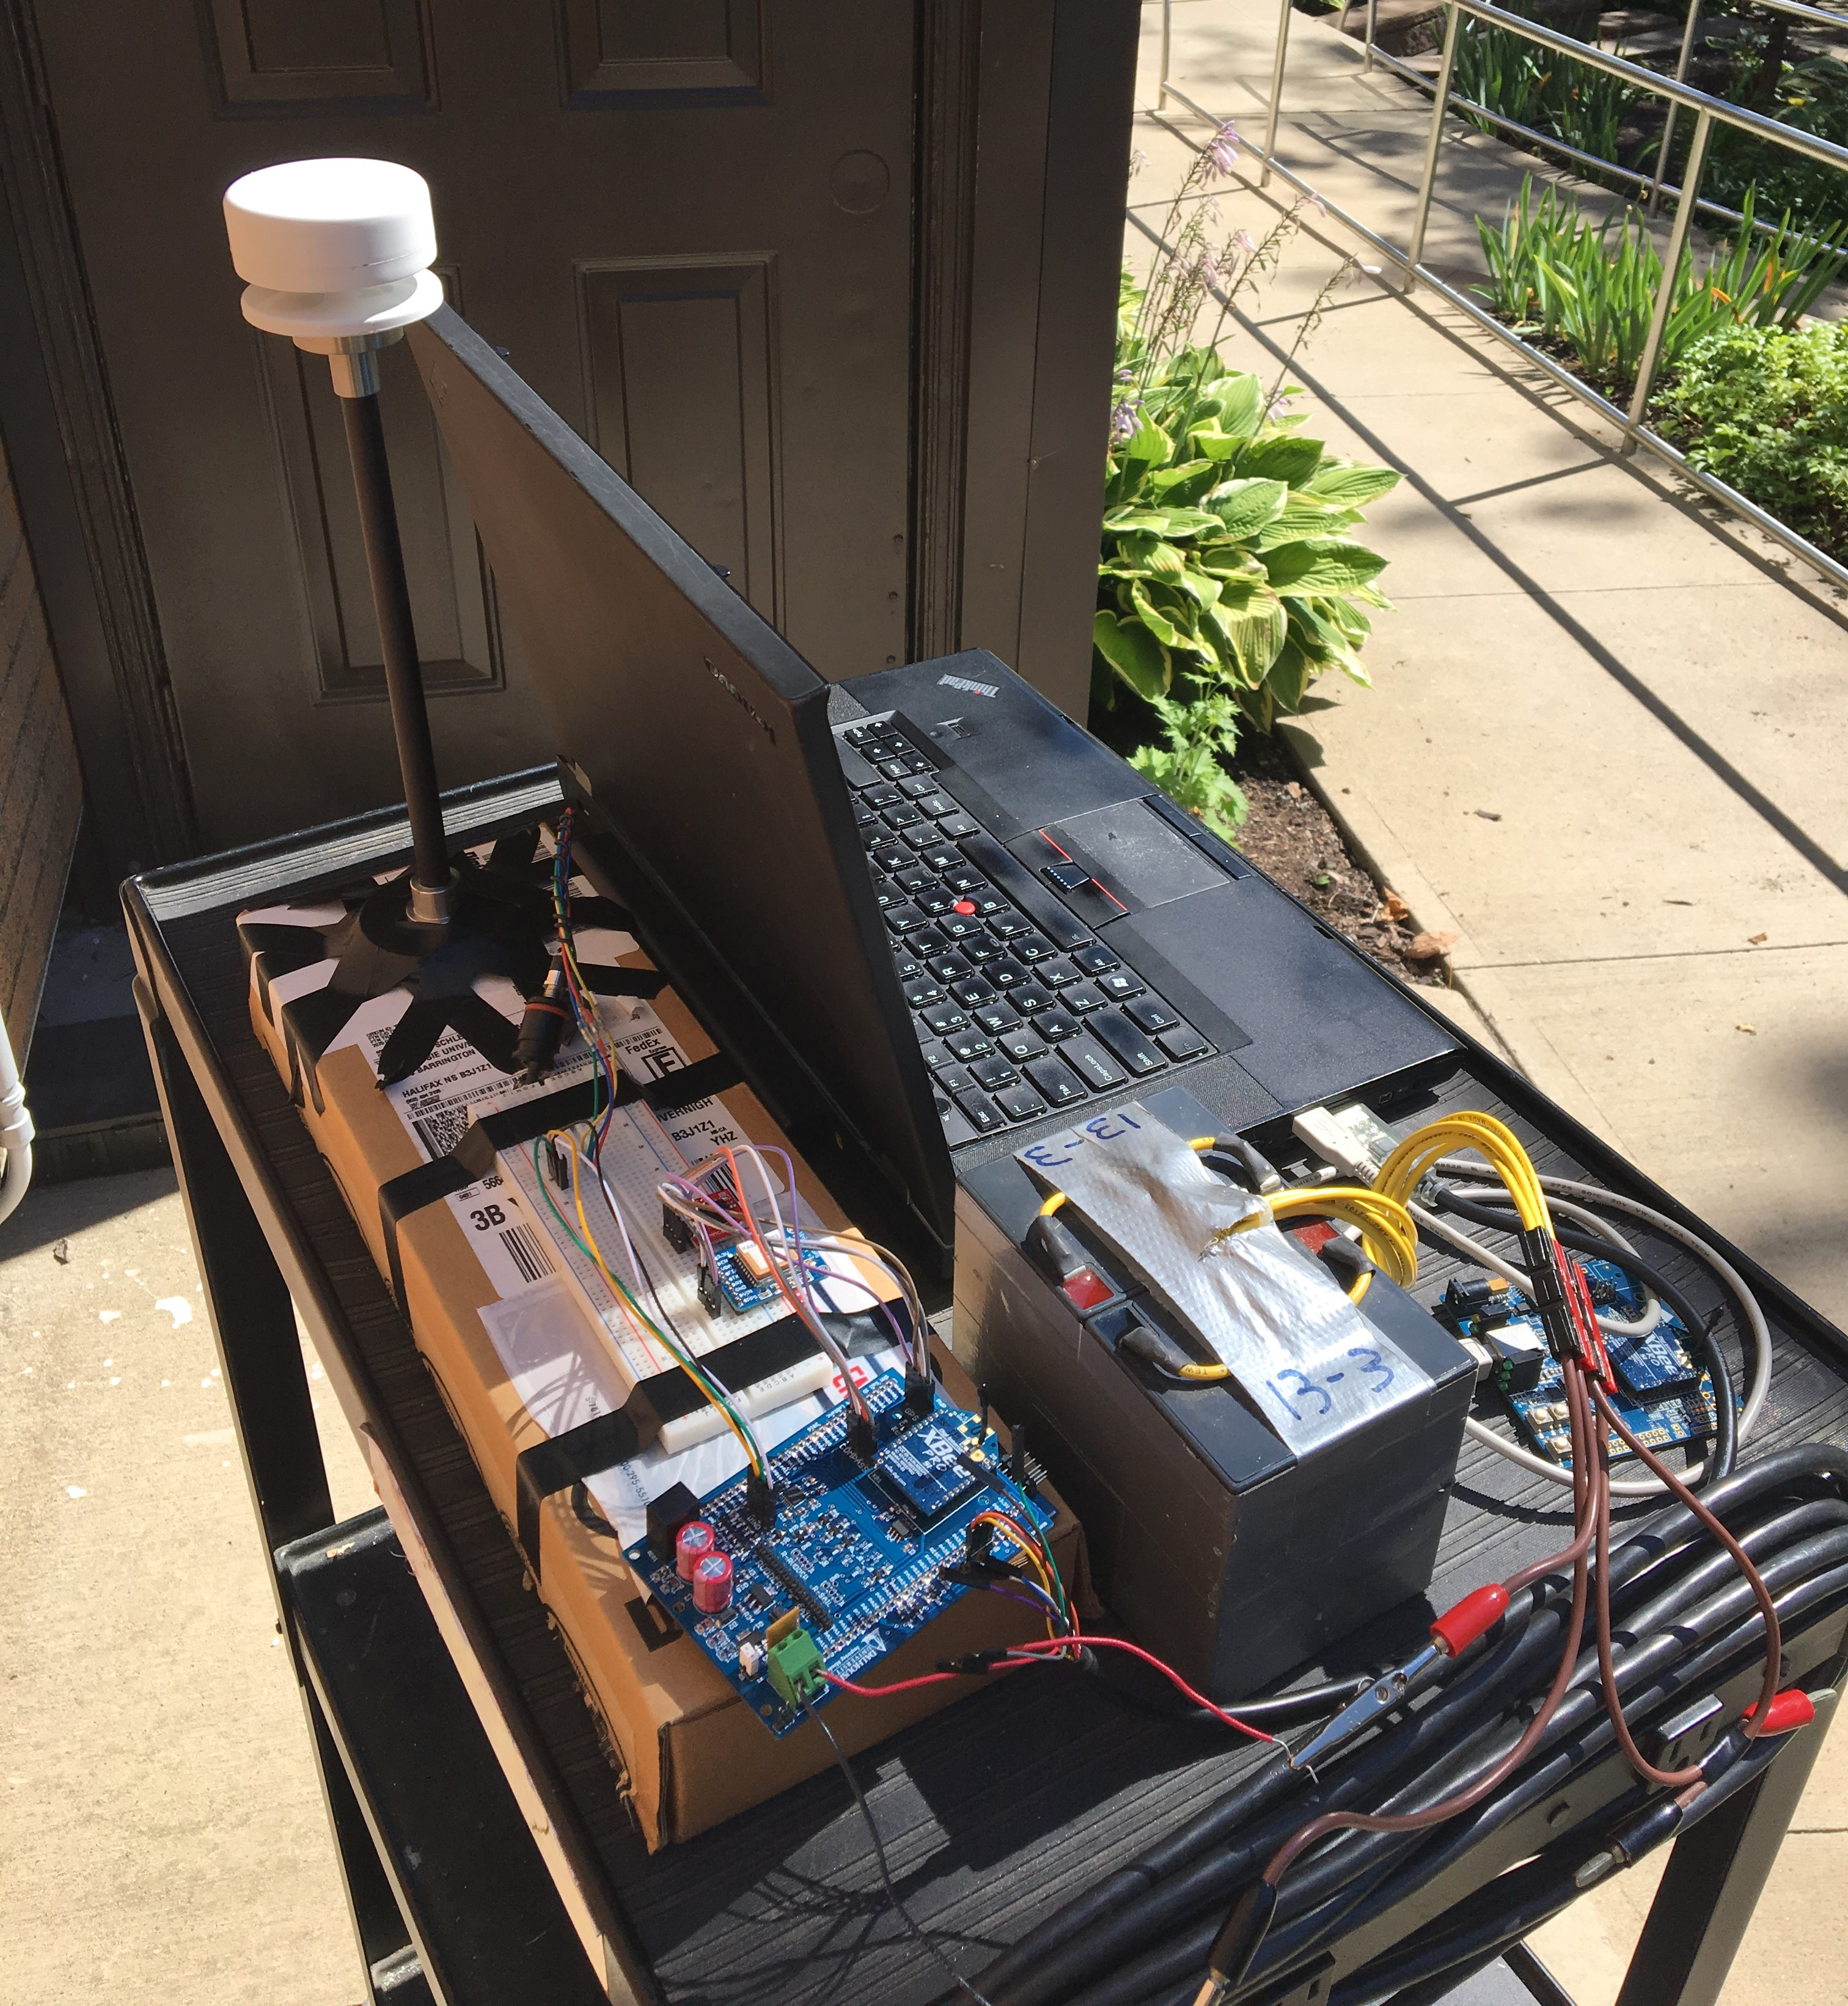
\includegraphics[width=0.5\textwidth]{figures/sailboat_cart1.jpg}
	\caption[Sailboat test cart]{\textsl{Sailboat test cart}}
	\label{fig:sail_cart}
\end{figure}

\clearpage

\section{Conclusion \& Recommendations}
This work term provided a challenging task -- design and implement a control system for an autonomous sailboat. 

\clearpage

\begin{thebibliography}{9}
	\bibitem{micro_rules}
	Microtransat Committee,
	\emph{The Microtransat Challenge: Rules},\\*
	http://microtransat.org/rules.php.
	2016.
	
	\bibitem{micro_main}
	Microtransat Committee,
	\emph{The Microtransat Challenge},\\*
	http://microtransat.org/index.php.
	2016.
	
	\bibitem{micro_map}
	Microtransat Committee,
	\emph{The Microtransat Challenge: 2016 Course (West to East)},\\*
	http://microtransat.org/2016.php.
	2016.
	
\end{thebibliography}

\clearpage

\appendix
\section{Select Code Listings}

\lstinputlisting[language=c, firstline=275, lastline=292, caption={Control timer callback function}, label={list:timer_tick}]{"../../src/sail_ctrl.c"}

\lstinputlisting[language=c, firstline=35, lastline=55, caption={Enumerated control states}, label={list:ctrl_enum}]{"../../src/sail_types.h"}

\clearpage

\lstinputlisting[language=c, firstline=15, lastline=64, caption={GPS module interface}, label={list:gps_interface}]{"../../src/sail_gps.h"}

\clearpage

\lstinputlisting[language=c, firstline=16, lastline=58, caption={Wind module interface}, label={list:wind_interface}]{"../../src/sail_wind.h"}

\clearpage

\lstinputlisting[language=c, firstline=14, lastline=55, caption={Compass module interface}, label={list:comp_interface}]{"../../src/sail_comp.h"}

\end{document}          
